\documentclass[12pt,a4paper]{scrartcl}
\usepackage[utf8]{inputenc}
\usepackage[T1]{fontenc}
\usepackage{lmodern}
\usepackage[ngerman]{babel}
\usepackage{amsmath}
\usepackage[automark, headsepline, footsepline]{scrpage2}
\usepackage{graphicx}
\usepackage{url}
\usepackage[hidelinks]{hyperref}
\usepackage{caption}

\widowpenalty10000
\ihead[]{}
\chead[]{\headmark}
\ohead[]{}
\ifoot[]{}
\cfoot[\pagemark]{\raisebox{-.2cm}{\thepage}} 
\ofoot[]{}
\pagestyle{scrheadings}
\setkomafont{pageheadfoot}{\normalfont\small\sf}

\author{Jan Philipp Vogtherr \& Timmy Schüller\vspace{0.5cm}}
\title{
\includegraphics[scale=0.8]{unilogo.pdf}\vspace*{1cm}
\mbox{Projekt OScillate:} \mbox{Ein Modell der Osnabrücker} Buslinien 11 und 21\vspace{0.3cm}}
\date{Universität Osnabrück \\
Im Rahmen der Veranstaltung \glqq Regelbasierte Modellierung\grqq \\
\vspace*{0.4cm}
Wintersemester 2013/2014 \\
\today}

\begin{document}

\maketitle
\thispagestyle{empty}
\newpage
\tableofcontents
\newpage

\section{Motivation}
Als Student der Universität oder Hochschule in Osnabrück steht man täglich vor einer schwierigen Entscheidung, wenn man den Campus am Westerberg erreichen möchte. Der Weg dorthin beinhaltet für viele Studenten eine Busfahrt vom zentralen Verkehrsknotenpunkt, dem Neumarkt, zum Zielort, wobei es dort zwei verschiedene Buslinien gibt, die jeweils Vor- und Nachteile mit sich bringen. Die Buslinie 21 fährt einen kleinen Umweg, sodass sie langsamer ist, als die konkurrierende Buslinie 11. Außerdem fährt die 21 mit einem 15-Minuten Takt weniger oft als die 11 mit einem 10-Minuten Takt. Allerdings hält die 11 nicht direkt an der Haltestelle vor der Uni, sondern zieht immer einen Fußweg von bis zu fünf Minuten mit sich. Zu bestimmten Tageszeiten kann eine Buslinie besonders überfüllt sein, während die andere eher leer ist. Die zu Beginn angesprochene Entscheidung ist also nun: \glqq Fahre ich heute mit der 11, oder der 21?\grqq

Das im folgende vorgestellte Projekt OScillate beschäftigt sich mit ebendieser Problematik. Im Rahmen der Veranstaltung \glqq Regelbasierte Modellierung\grqq~wurde ein agentenbasiertes Modell erstellt, das die Entscheidungsdynamik dieser Fragestellung nachstellen soll. Zu finden ist das Projekt unter \url{https://github.com/jvogtherr/OScillate}.

In \autoref{design} werden zunächst grundlegende Designentscheidungen erläutert. Darauf basierend geht es in \autoref{impl} um die Umsetzung der Ideen, direkt gefolgt von einer Auswertung der daraus resultierenden Ergebnisse in \autoref{erg}. Abschließend diskutiert \autoref{fazit} den Verlauf des Projektes, sowie die erhaltenen Ergebnisse.

\section{Design}\label{design}
Der Modellzweck ist explorativ und lässt sich in folgender Leitfrage zusammenfassen: \glqq Welche Faktoren haben einen Einfluss auf die Wahl der Buslinie?\grqq 

Das Modell ist insgesamt sehr auf die Situation in der realen Welt zugeschnitten und lässt sich kaum auf andere übertragen. Außerdem verwendet das Modell sowohl eine sehr hohe zeitliche, als auch räumliche Auflösung, daher kann der Abstraktionsgrad insgesamt als realistisch eingestuft werden. Die komplexe Entscheidung der homogenen Agenten, der Studenten, trägt ebenfalls dazu bei und führt zu einer hohen individuellen Komplexität. Funktionale Heterogenität gibt es in direktem Sinne nicht, weil es außer den Studenten keine weiteren Akteure gibt. Die Interaktionen der Studenten untereinander beschränken sich auf simple Beobachtung der Handlungen der anderen Akteure, echte Interaktionen gibt es nicht.

\section{Implementierung}\label{impl}
Die zentralen Elemente des Modells sind Studenten als Agenten des Systems und die Busverbindung, die die Umwelt darstellt, in der die Agenten selbstständig über ihr Handeln bestimmen können. Zunächst werden die verwendeten Mechanismen beider Elemente respektiv erklärt. Anschließend wird die Implementierung im Detail besprochen.

\subsection{Agent: Student}\label{agent}
Ein Student soll sich täglich selbstständig von seiner Wohnung zum Neumarkt bewegen und sich dort für eine Buslinie entscheiden, mit der er zur Universität fährt. Dort angekommen soll er für die Dauer einiger Vorlesungen auf dem Campus bleiben und anschließend von der Bushaltestelle an der Universität zurück zum Neumarkt fahren, wobei er erneut eine Buslinie auswählen muss. Zur Vereinfachung wurden hier die zwei zuvor angesprochenen Haltestellen der beiden Linien zusammengefasst. 
Das Ziel des Studenten ist die Auswahl einer Buslinie unter Berücksichtigung seiner persönlichen Eigenschaften, mit der er eine möglichst kurze Reisedauer und wenig Wartezeit an den Haltestellen erreicht.

Die Studenten in dem Modell unterscheiden sich im Zeitpunkt ihres Erscheinens und ihrer Aufenthaltsdauer in der Universität. So kommen einige Studenten besonders früh und hören viele Vorlesungen, während andere Studenten erst spät kommen und nur wenige Vorlesungen hören, bevor sie wieder nach Hause fahren.

Jeder Student hat eine bevorzugte Buslinie, die sich über die Zeit ändern kann. Nach jeder Busfahrt evaluiert der Student seine Entscheidung und merkt sich das Ergebnis seiner Überlegungen, sodass er die Zufriedenheit des Vortages bei jeder Entscheidung aufs neue mit einbeziehen kann. Im Modell wird die bevorzugte Buslinie als Parameter des Studenten dargestellt. Zu Beginn sind die bevorzugten Buslinien unter allen Studenten zufällig verteilt - mit Ausnahme der Erstsemesterstudenten, deren bevorzugte Buslinie zu Beginn stets die Linie 21 ist. Die Anzahl der \glqq Ersties\grqq~ kann als Simulationsparameter variiert werden.

Bei der Entscheidungsfindung der Buslinie kommt ein Parameter zum Tragen, der im Folgenden als der \glqq Sozialfaktor\grqq~bezeichnet wird. Dieser Parameter ist unter den Studenten zufällig verteilt und modelliert die Bereitschaft eines Studenten, in einen bereits sehr vollen Bus einzusteigen. Dies kann verschiedene Situationen der echten Welt darstellen. Beispielsweise könnte ein niedriger Sozialfaktor zeigen, dass der Student in einer größeren Gruppe unterwegs ist und diese Gruppe nur dann in einen Bus einsteigt, wenn alle Mitglieder der Gruppe einen Sitzplatz bekommen können. Im Gegensatz dazu könnte ein hoher Sozialfaktor  einen allein fahrenden Studenten darstellen, der auch bereit ist, in einen überfüllten Bus einzusteigen.

\subsection{Umwelt: Busverbindung}\label{bus}
Die Busverbindung verwaltet die Haltestellen am Neumarkt und der Universität, sowie alle Busse, die diese Haltestellen anfahren. Den Studenten wird somit die Möglichkeit gegeben sich an einer Haltestelle anzustellen, auf einen beliebigen Bus zu warten und mit diesem Bus zum Ziel zu fahren. Nach Ablauf der Fahrtzeit muss der Student wieder aus dem Bus aussteigen und von der Haltestelle nach Hause bzw. in die Universität gehen. 

Um der Realität etwas näher zu kommen gibt es nicht nur Studenten die Bus fahren, sondern es wird mithilfe einer Polynomfunktion eine \glqq Hintergrundlast\grqq~ modelliert. Die verwendete Funktion besitzt ein Maximum morgens und eines zum Feierabendverkehr und beschreibt die Anzahl der Fahrgäste in einer Buslinie, die keine Studenten sind.

\begin{figure}[ht!]
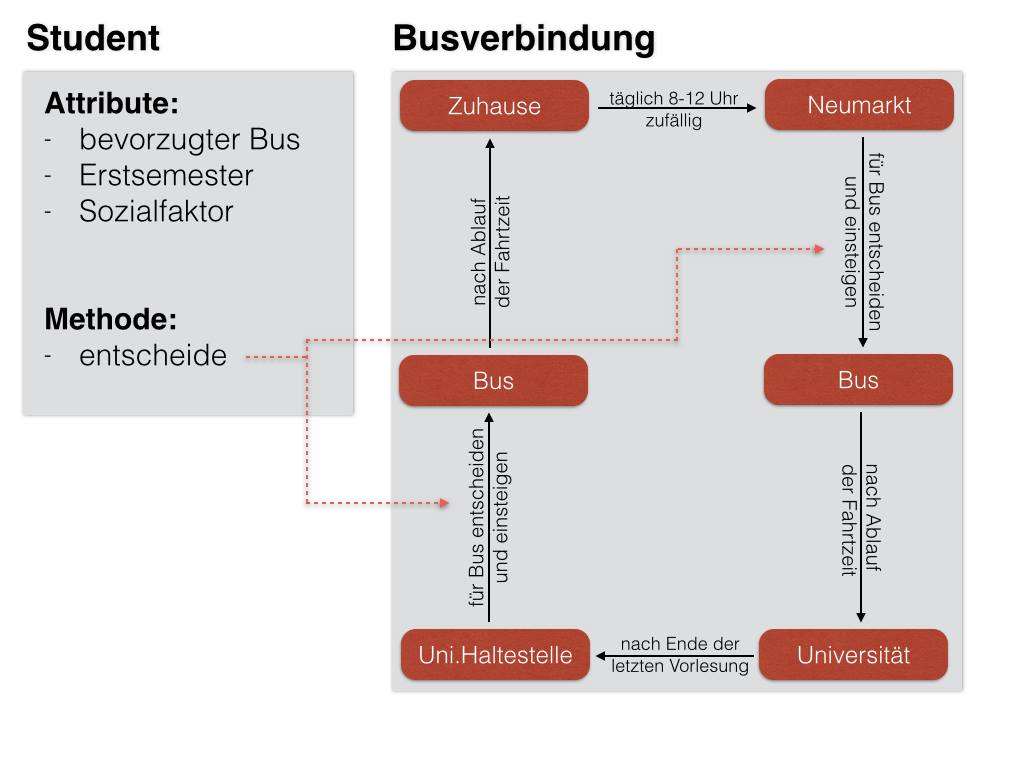
\includegraphics[scale=0.4]{Ablaufdiagramm.jpg}
\caption{Tagesablauf eines Studenten in Projekt OScillate}
\label{ablauf}
\end{figure}


\subsection{Implementierung mithilfe von Repast Symphony}\label{repast}

Das Modell wird mit dem Modellierungswerkzeug Repast Simphony in Java implementiert und ausgewertet. Zunächst müssen Umwelt und Agenten als Java-Klassen programmiert werden. Jede Simulation muss eine Klasse beinhalten, die das Interface \textit{ContextBuilder} implementiert. In diesem Fall ist dies die Klasse \textit{OScillateBuilder}. Die Methode \textit{build} soll nun die Umwelt initialisieren und die Agenten in der Umwelt ansiedeln, um die Simulation starten zu können. Zunächst werden die Simulationsparameter, die der Nutzer in der graphischen Oberfläche spezifizieren kann, ausgelesen und für die spätere Verwendung vorbereitet. Anschließend werden sowohl eine neue Busverbindung als auch die gewünschte Anzahl an Studenten erzeugt.

Die Busverbindung enthält drei Listen und eine Sammlung von Schlüssel/Wert-Paaren (im Folgenden Map). Die Listen enthalten alle Studenten die sich Zuhause, am Neumarkt oder an der Haltestelle an der Universität aufhalten. Die Map enthält alle Studenten, die sich zur Zeit in der Universität befinden, zusammen mit der entsprechenden restlichen Aufenthaltsdauer.

Außerdem enthält die Busverbindung zwei Instanzen der Klasse \textit{Bus}, von der jede eine der beiden Buslinien 11 und 21 darstellt. Ein \textit{Bus}-Objekt modelliert alle Busse, die derzeit auf der entsprechenden Linie fahren, mit allen Fahrgästen, die in einem der Busse sitzen. Umgesetzt wird dies mit Hilfe einer Map als Speicherstruktur. In dieser Map werden, ähnlich wie bei der Universität, die Studenten im Bus mit ihrer restlichen Fahrtzeit und ihrer Fahrtrichtung gespeichert. Somit kann man mit den beiden Objekten alle Studenten darstellen, die sich zur Zeit in irgendeinem Bus befinden.

Wenn ein Student also vom Neumarkt zur Uni fährt, so wird er zunächst in der \glqq Neumarkt-Liste\grqq~der Busverbindung eingeordnet, bis er in einen Bus einsteigt. Dann wird er in die Map des Busses eingetragen und verbleibt dort, bis seine Fahrtzeit abgelaufen ist. Nun verlässt er den Bus an der Universität und wird mit seiner Aufenthaltszeit in die Map der Universität eingetragen. Nachdem auch hier seine Aufenthaltszeit abgelaufen ist, wird er in die entsprechende Liste der Haltestelle an der Universität eingetragen, bis er dort in einen Bus steigt. In diesem Bus wird er wiederum mit seiner verbleibenden Fahrzeit eingetragen und verweilt im Bus, bis diese abgelaufen ist und er somit am Ende des Tages am Neumarkt ankommt und nach Hause geht, wo er in die entsprechende \glqq Zuhause-Liste\grqq~eingetragen wird, bis er am nächsten Morgen wieder zum Neumarkt geht. Zusammenfassend kann man sagen, dass alle Mengen von Studenten mit unbestimmter Aufenthaltszeit an ihrem aktuellen Ort als Liste und alle Mengen von Studenten mit begrenzter Aufenthaltszeit an ihrem aktuellen Ort als Map gespeichert werden.

Die Klasse \textit{Student} speichert und abstrahiert die jeweiligen Eigenschaften des Studenten, die bei seiner Erstellung angegeben werden und sich im Laufe des Modells entwickeln. So kann beispielsweise der Sozialfaktor zu Beginn festgelegt werden. Die wichtigste Fähigkeit des Studenten ist die Entscheidung, die er vor jeder Busfahrt treffen muss. Dargestellt wird diese mit der Methode \textit{entscheide}. Übergeben werden die Informationen, welche Buslinie gerade an der Haltestelle steht und wie voll die jeweiligen Busse sind, wobei letzteres durch die Asynchronität des Modells möglich wird. So kann der Student in einen Bus einsteigen oder warten und vorerst gar nichts tun. Alle Möglichkeiten der Entscheidung werden überprüft und diejenige mit der höchsten Priorität wird ausgewählt, sodass der Student seine Lage nach seinem Wissen optimal einschätzt und effizient handelt. 

Eine wesentliche Rolle spielt hierbei der Sozialfaktor. Ist ein Bus voller als es der Sozialfaktor eines Studenten erlaubt, so wird er nicht einsteigen, wobei durch den maximalen Sozialfaktor indirekt der Parameter der Buskapazität eingeführt wird.

Während \glqq normale\grqq~Studenten dazu in der Lage sind mit einem Bus zu fahren, die nicht ihrem bevorzugten Bus entspricht, beispielsweise wenn dieser zu voll oder einfach gerade nicht da ist, dürfen die zuvor bereits erwähnten \textit{Ersties} dies nicht. Ein Erstie wird zu einem \glqq normalen\grqq~Studenten, wenn er mit der 21 so unzufrieden ist, dass der bevorzugte Bus wechselt. Er wird, praktisch gesprochen, irgendwann experimentierfreudig und findet heraus, dass es eine weitere Linie gibt.

Eine Besonderheit der Modellierung mit Repast Simphony sind die sogenannten \textit{ScheduledMethods}. Durch eine entsprechende \textit{Annotation} im Java-Code kann man eine Methode zu einem definierten Zeitpunkt im Programmablauf ausführen lassen. Repast Simphony rechnet in \textit{Ticks} als Zeitschritt. Im Modell entspricht ein Tick fünf Minuten. Somit ergeben sich für die Buslinie 11 zum Beispiel eine Fahrtzeit von zwei Ticks, während die Buslinie 21 eine Fahrtzeit von drei Ticks hat, um grobe Anlehnungen an die Realität zu erhalten. Die Busverbindung ist das einzige Objekt in der Simulation, das solche Methoden enthält und fungiert somit als eine Art Managerklasse, die den anderen Objekten zu jedem Zeitpunkt Anordnungen gibt. Das beinhaltet zum Beispiel das Aktualisieren der verbleibenden Aufenthalts- und Fahrtzeiten der Studenten in der Universität und in den Bussen, sowie das Ein- und Aussteigen an den Haltestellen. Außerdem bietet die Busverbindung die nötigen Schnittstellen zur graphischen Auswertung der Simulation, in dem die Klasse verschiedene Methoden für statistische Angaben zum Modell bietet. 

\section{Auswertung}\label{erg}
Im Folgenden werden einige Ergebnisse der Modellierung anhand von Grafiken erläutert. Mithilfe der Parameterkonfiguration lassen sich verschiedene Szenarien konstruieren, um das Modell auszuwerten. In diesem Kapitel wird zuerst das realitätsnahe Standardszenario vorgestellt, das einen Einblick in das Modellverhalten bietet. Anschließend wird in einem extremen Szenario gezeigt, welches Verhalten bei gleichbleibender Buskapazität aber deutlich erhöhter Studentenzahl eintritt.

\subsection{Standardszenario}\label{s1}
\begin{figure}
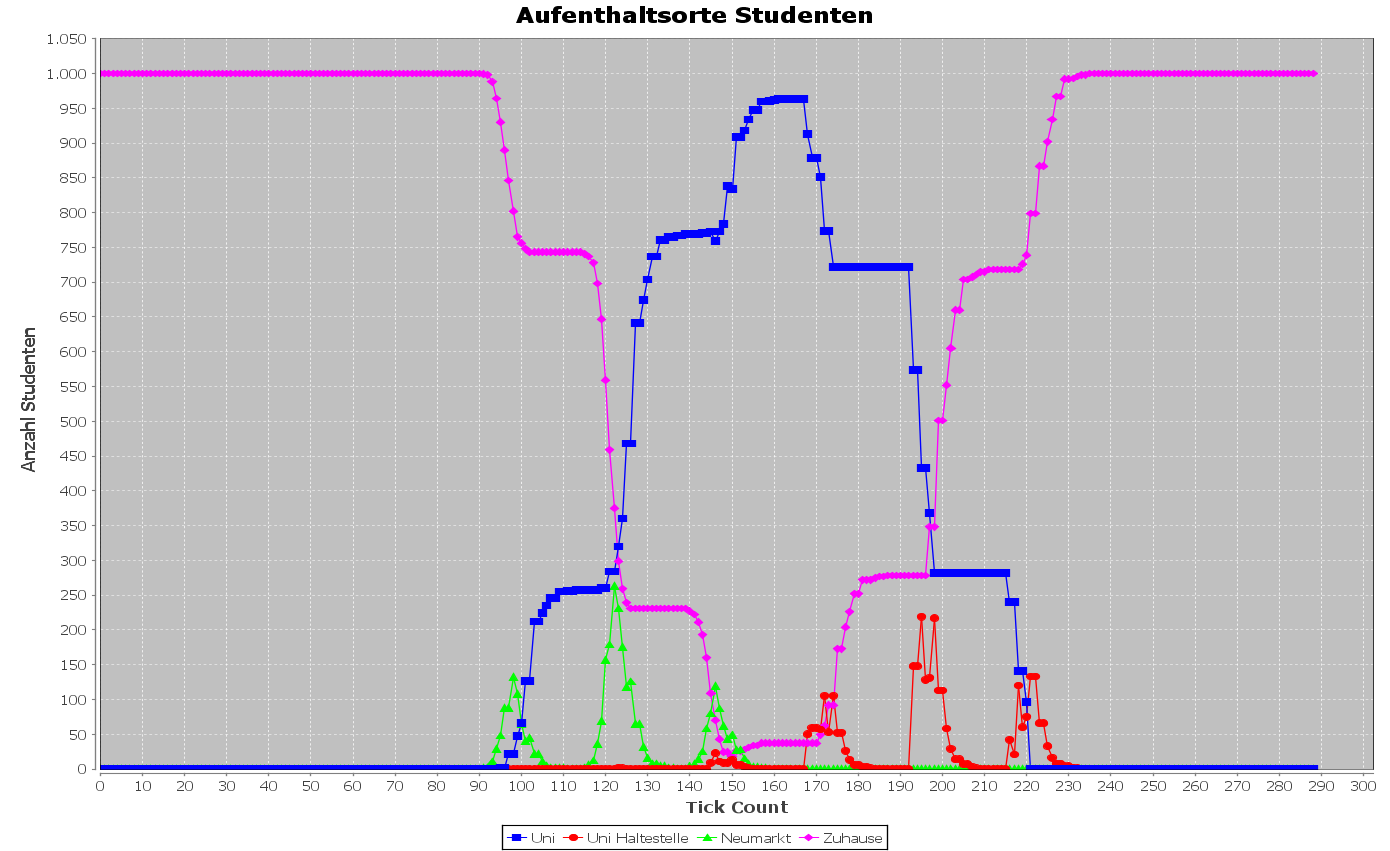
\includegraphics[scale=0.4]{Standardszenario_Aufenthaltsorte.png}
\caption{Standardszenario: Aufenthaltsorte der Studenten}
\label{s1g1}
\end{figure}

In \autoref{s1g1} kann man einen Tagesdurchlauf der Simulation erkennen. Dabei stellt jeder Graph die Anzahl der Studenten an einem bestimmten Aufenthaltsort im System dar. Betrachtet man den pinken Graphen, so kann man erkennen, zu welchen Uhrzeiten die Studenten typischerweise den Weg zur Universität beginnen. In drei Stoßzeiten laufen die Studenten zum Neumarkt, jeweils um acht Uhr, um zehn Uhr und um zwölf Uhr. Die Startzeit eines Studenten ist um eine der drei Stoßzeiten normalverteilt, sodass einige bereits früher als acht Uhr das Haus verlassen, während einige auch erst deutlich nach zwölf Uhr losgehen. 

Analog dazu kann man erkennen, dass die Studentenwellen, die zu den drei Stoßzeiten losfahren, ebenfalls kurze Zeit später in solchen Wellen an der Universität ankommen (blauer Graph). Das bedeutet, dass es zu keinen unerwarteten Verzögerungen im Busverkehr gekommen ist. Ähnlich wie beim Hinweg reisen die Studenten nach einem ähnlichen Muster von der Universität nach Hause, nämlich nach Ende von vordefinierten Vorlesungsblocks. So hören einige Studenten nur wenige Vorlesungen und fahren früh, während andere lange bleiben und erst am Ende des Tages nach Hause fahren. 

Der grüne und der rote Graph zeigen die Anzahl der Studenten am Neumarkt und an der Unihaltestelle. Beide verhalten sich prinzipiell ähnlich. Zu jeder Stoßzeit schlagen die Graphen nach oben aus. Das zeigt, dass zu den Zeitpunkten viele Studenten an der Haltestelle auf einen Bus warten müssen. Nach sehr kurzer Zeit hat die Buslinie alle Studenten von der Haltestelle abgeholt und die Situation beruhigt sich schnell wieder.
Insgesamt kann man im Standardszenario also das Prinzip der Simulation gut erkennen und es treten keine Probleme oder unerwartetes Verhalten auf.

\begin{figure}
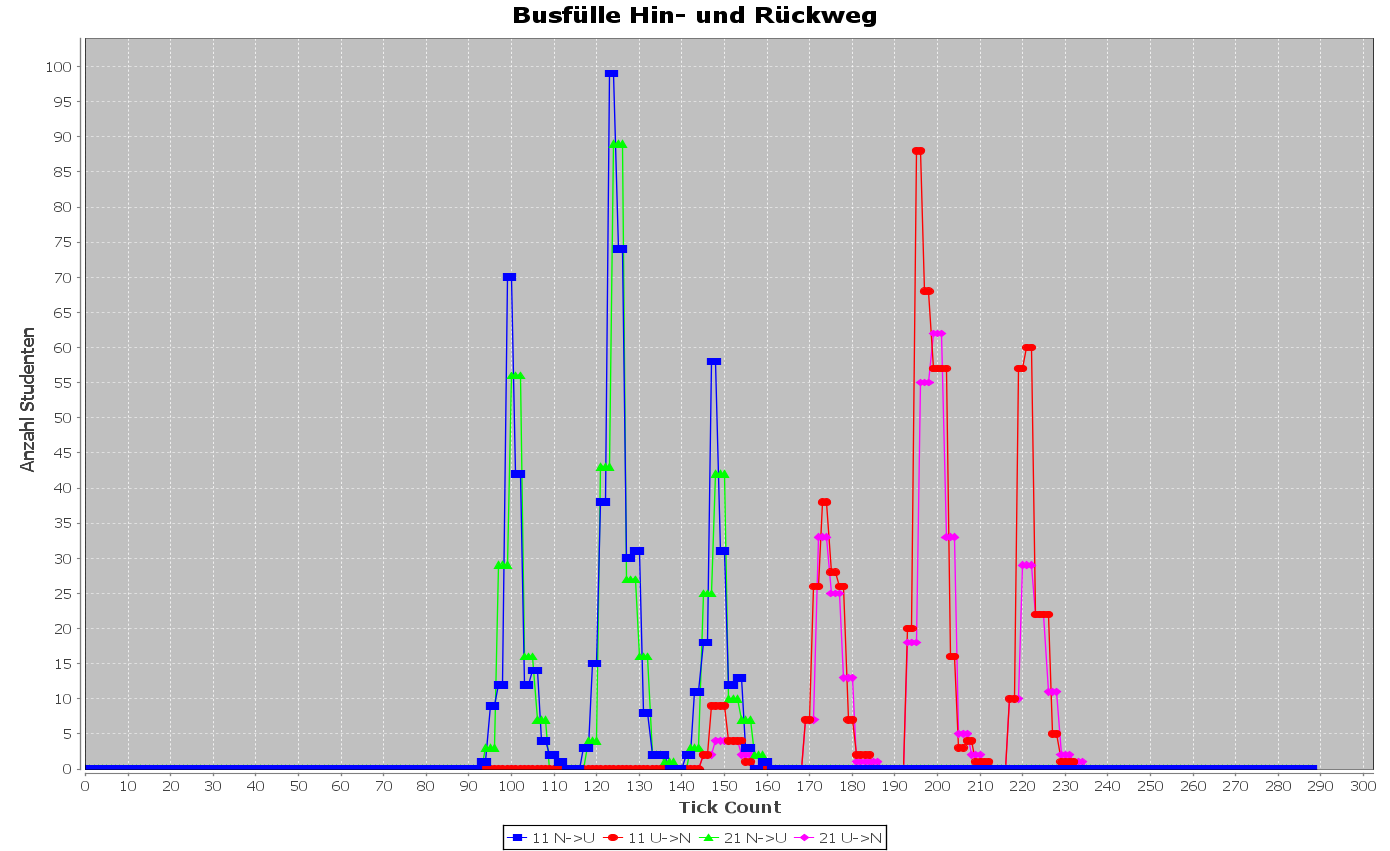
\includegraphics[scale=0.4]{Standardszenario_Busse.png}
\caption{Standardszenario: Anzahl von Studenten in verschiedenen Bussen}
\label{s1g2}
\end{figure}

\autoref{s1g2} ist ebenfalls ein Diagramm, das das Standardszenario darstellt. Der blaue und grüne Graph zeigen die Anzahl der Studenten im Bus 11 und im Bus 21 auf dem Weg zur Universität. Der rote und der pinke Graph zeigen die Anzahl der Studenten im Bus 11 und im Bus 21 auf dem Weg von der Universität zurück zum Neumarkt. Zu den bereits genannten Stoßzeiten zu Beginn des Tages um acht, zehn und zwölf Uhr kann man die Graphen für die Busfülle der Linien in Richtung Universität sehen. Dies sind die Studenten, die morgens zur Uni fahren. Man kann erkennen, dass beide Buslinien ähnlich genutzt werden, wobei man dennoch sagen kann, dass die Linie 11 stärker genutzt wird. 

Auf dem Rückweg von der Universität ist die Situation ähnlich, mit dem Unterschied, dass es nicht drei, sondern vier Stoßzeiten gibt, von denen die erste die mit Abstand kleinste ist. Auch hier ist das Fahrverhalten der Studenten ähnlich, wobei die Buslinie 11 tendenziell mehr genutzt wird. 
Zu erklären ist das in diesem Szenario durch die kürzere Fahrtzeit der 11. Da der Bus öfter kommt und insgesamt kürzer fährt, ist er in der Lage, mehr Studenten aufzunehmen als die Buslinie 21. Da zu Beginn der \textit{bevorzugter Bus} Parameter zufällig verteilt ist, fahren zu Beginn auch sehr viele Studenten mit der 21. Über längere Zeit wechseln einige Studenten von der Buslinie 11 zur 21, da die 11 zu oft zu voll wird, was in diesem Diagramm nicht mehr zu erkennen ist. Über die Zeit kann sich ein Gleichgewicht einstellen.

\subsection{Szenario: Zu viele Studenten}\label{s2}

\begin{figure}
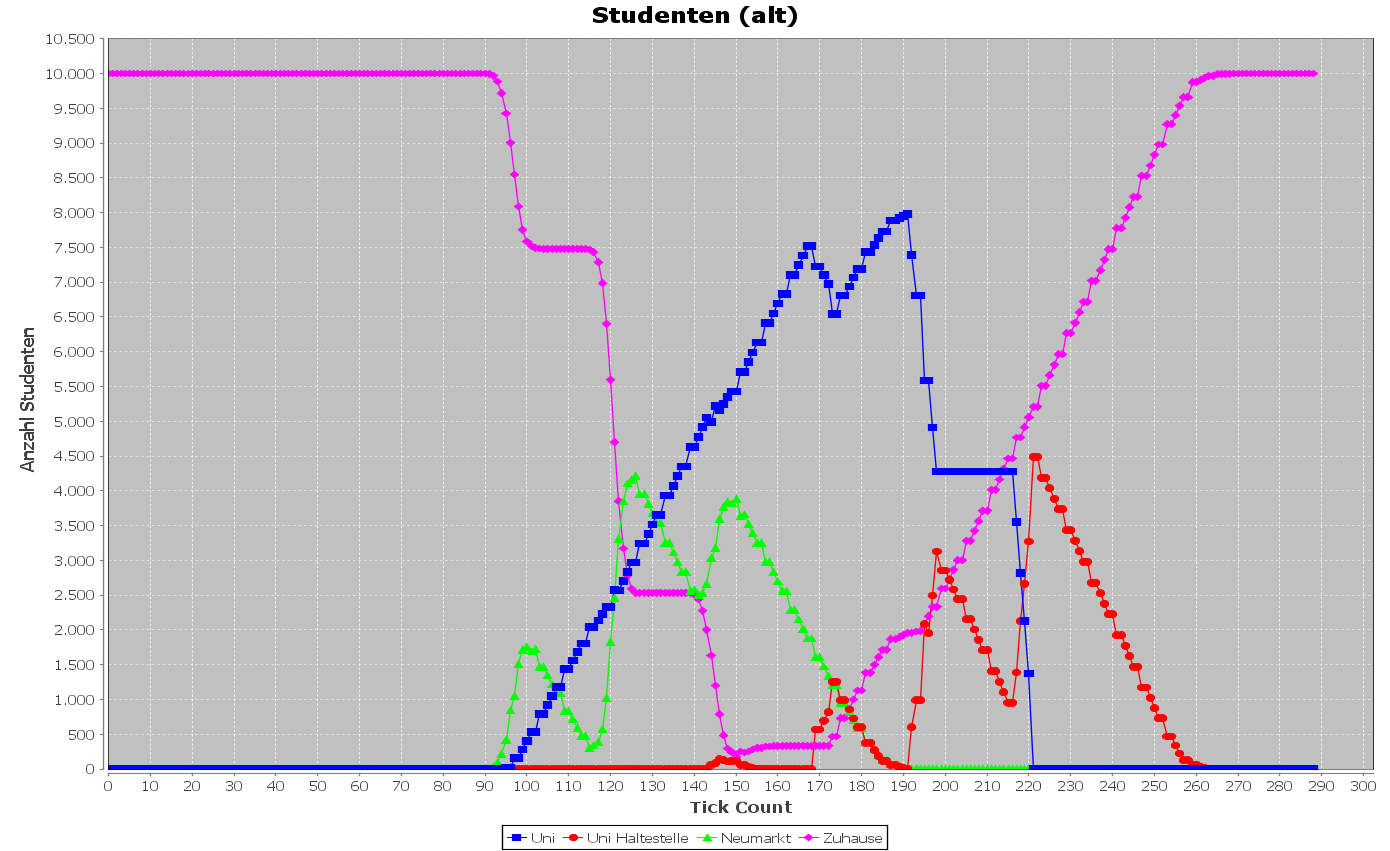
\includegraphics[scale=0.4]{Viele_Studenten_Aufenthaltsorte.png}
\caption{Szenario \glqq Zu viele Studenten\grqq : Aufenthaltsorte der Studenten}
\label{s2g1}
\end{figure}

In \autoref{s2g1} kann man, ähnlich wie in \autoref{s1g1}, erkennen, wie viele Studenten zu welchem Zeitpunkt an welchem Ort sind. Besonders ist hierbei, dass die Anzahl der Studenten zehn mal so hoch gewählt ist, wie im Standardszenario, während die Buskapazitäten gleich geblieben sind. Insgesamt gibt es nun also deutlich zu viele Studenten für die Busverbindung. Dies äußert sich an den Wartezeiten am Neumarkt und an der Bushaltestelle an der Universität.
Der grüne Graph zeit die Anzahl der Studenten am Neumarkt. Wie man sehen kann, sinkt der Graph  nach dem ersten Hochpunkt langsam. Dies bedeutet, dass zu Beginn sehr viele Studenten an den Neumarkt kommen, dort auf einen Bus warten und schließlich losfahren. Bis der Anstieg zum zweiten Hochpunkt losgeht, sind aber noch nicht, wie im Standardszenario, alle Studenten vom Neumarkt aufgebrochen, bevor die zweite Stoßzeit beginnt, sodass sich in diesem Fall zwei Stoßzeiten überlagern. Das hat zur Folge, dass jeder Bus, egal ob 11 oder 21, der am Neumarkt ankommt, so viele Studenten mitnimmt, wie er kann. Zu beobachten ist dies bei dem blauen Graphen, der zeigt, wie viele Studenten an der Universität angekommen sind. Der Bus steigt linear, was die Erklärung für das Verhalten am Neumarkt bestätigt. Jeder Bus der an der Uni ankommt ist maximal besetzt und es dauert eine gewisse Zeit, bis alle Studenten vom Neumarkt zur Universität gelangt sind. Gegen Ende sind die Busse dann auch nicht mehr maximal besetzt und es stellt sich wieder ein annähernd normales Verhalten ein. 
Die Dynamik der Rückfahrt ist in diesem Fall analog. Die Bushaltestelle an der Universität wird nach den Vorlesungsendzeiten stark überfüllt, sodass selbst spät abends noch Studenten an der Haltestelle stehen und auf einen Bus warten müssen. 

\begin{figure}
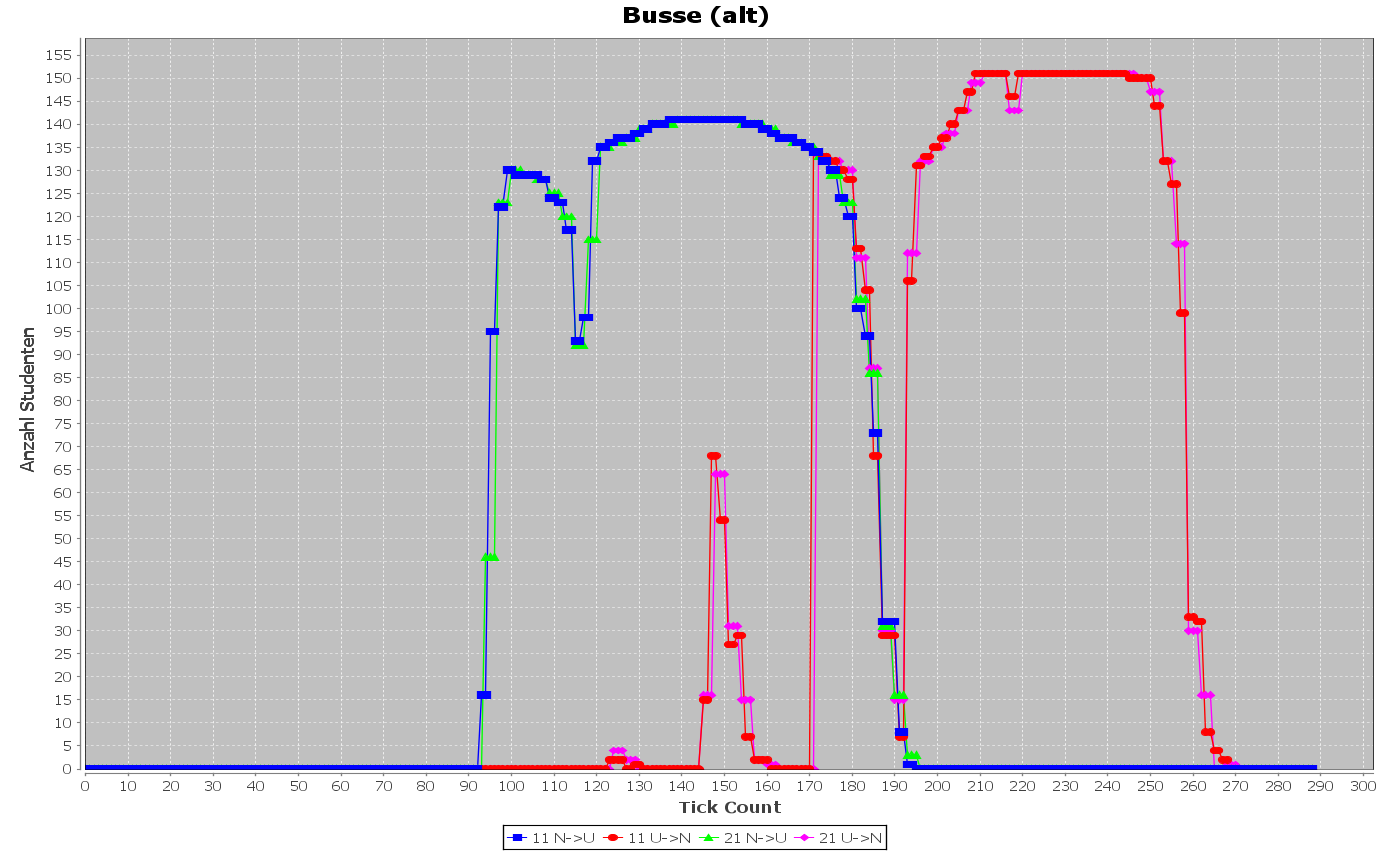
\includegraphics[scale=0.4]{Viele_Studenten_Busse.png}
\caption{Szenario \glqq Zu viele Studenten\grqq : Anzahl von Studenten in verschiedenen Bussen}
\label{s2g2}
\end{figure}

\autoref{s2g2} zeigt den Tagesablauf aus \autoref{s2g1} wieder aus der Perspektive der einzelnen Buslinien. In diesem Fall sind die Buslinien 11 und 21 ähnlich voll besetzt, was sich auch über mehrere Simulationen nicht ändert. Wie in \autoref{s1g1} gehören hier wieder jeweils der blaue und der grüne Graph zusammen und zeigen den Hinweg zur Universität, während der pinke und der rote Graph den Rückweg zeigen. Vergleicht man \autoref{s2g1} und \autoref{s2g2}, so kann man sehen, dass in diesem Fall die Buslinien während der Hin- bzw. Rückfahrtzeiten stets besetzt sind und keine Linie zu einem Zeitpunkt keine Fahrgäste hat. Besonders stark ist der Unterschied bei der zweiten und dritten Stoßzeit während der Hinfahrt und bei den beiden letzten Stoßzeiten der Rückfahrt. Hier ist für eine gewisse Zeit die Buskapazität dauerhaft erreicht und die Busse sind vollständig besetzt. Darüberhinaus kann man hier die Funktion der sonstigen Fahrgäste in invertierter Form erkennen, da die Busse immer möglichst voll besetzt werden und sie die Buskapazität in Abhängigkeit von der Zeit verringert.


\subsection{kurze Zusammenfassung}\label{graphenzsm}
Zusammenfassend kann man hier sagen, dass das Extremszenario die Entscheidung des Studenten unnötig macht. Egal wie die Entscheidung ausfällt, durch die große Anzahl der Studenten ist es rein zufällig, ob er früh einen Sitzplatz in einem beliebigen Bus bekommt und in die Universität oder nach Hause kommt, oder ob er für sehr lange Zeit warten muss. Erst wenn der Student eine echte Wahl hat, also in einem Szenario mit weniger Studenten pro Sitzplatz in den Bussen, kann man die Dynamiken des Systems erkennen und verstehen. Das bedeutet, dass eine Modellierung mit empirisch erhobenen Daten zur genauen Bestimmung der Konstanten im System, wie zum Beispiel Anzahl der Studenten oder anderer Fahrgäste in den Bussen, weiterführende Fragestellungen klären und realistische Einschätzungen geben kann.

\newpage

\section{Fazit}\label{fazit}
Das Projekt OScillate befasste sich mit der Modellierung der Entscheidung von Studenten aus Osnabrück, mit welcher der beiden Buslinien, die zur Verfügung stehen, sie zur Uni und wieder zurück fahren. Realisiert wurde dies durch ein agentenbasiertes Modell, das mit der Modellierungsumgebung Repast Simphony implementiert wurde und den Tagesablauf eines Studenten realistisch darzustellen versucht. 

Während man die Entscheidungen eines Studenten in der Simulation an einem Tag gut nachvollziehen kann, so ist der Erfolg des Lernprozesses des Studenten bezüglich seiner bevorzugten Buslinie über einen längeren Zeitraum nicht besonders gut erkennbar. Dies liegt vor allem an der sehr hohen zeitlichen Auflösung des Modells und dem damit verbundenen Rechenaufwand, der das Modell bereits nach wenigen Tagen zum Erliegen bringt.

Positiv zu bewerten ist, dass das Modell den insgesamt sehr kleinschrittigen Tagesablauf verhältnismäßig simpel implementiert und somit Raum für beliebige Erweiterungen bietet. So kann beispielsweise ein soziales Netzwerk verwendet werden, um die Beziehungen der Akteure untereinander zu modellieren und in die Entscheidungsdynamik mit einzubeziehen. In einer sehr abstrakten Form wird dieses Verhalten durch den Sozialfaktor modelliert, der bereits im Modell implementiert ist. Außerdem könnten die Anzahl der Busfahrgäste, die keine Studenten sind, und die Anzahl der Studierenden, die Busse nutzen, durch eine empirische Datenerhebung besser dargestellt werden, um der Realität noch näher zu kommen. Dadurch entwickelt sich das Modell vom Verständnismodell weiter zum Vorhersagemodell, das mit echten Daten und Beobachtungen als Grundlage eine plausible Vorhersage für die Zukunft geben könnte. Dafür würde sich auch eine Implementierung in einer leistungsfähigeren Umgebung lohnen, um Daten über einen größeren Zeitraum berechnen zu lassen. 

Abschließend kann man sagen, dass der Projektablauf generell zufriedenstellend war. Nachdem zunächst ein lauffähiges Modell nach dem \textit{KISS}-Prinzip erstellt wurde und sukzessive erweitert wurde, war schnell absehbar, dass das Modell eher dem Verständnis einer Dynamik aus der echten Welt geben könnte, als eine exakte Modellierung dieser Dynamik zu explorieren. Dennoch konnte die grundlegende und zunächst irrtümlicherweise simpel erscheinende Leitfrage geklärt werden, welche Faktoren Einfluss auf die Entscheidung eines Studenten haben.
Eine weiterführende Fragestellung wäre nun, wie genau die Einflussfaktoren auf den Studenten wirken. Gelöst werden könnte eine solche Frage, wie bereits erwähnt, durch ein Vorhersagemodell, das die zugrundeliegende Funktionsweise dieses Modells aufgreift und darüber hinaus empirische Daten für genaue Prognosen verwenden sollte.
\end{document}
